\documentclass{jsarticle}
\usepackage[top=20truemm,bottom=20truemm,left=25truemm,right=25truemm]{geometry}
\usepackage{amsmath,ascmac,url,amsfonts,bm,here,algorithmic,algorithm,amsthm,color}
\usepackage[dvipdfmx]{graphicx}
\newcommand{\argmax}{\mathop{\rm argmax}\limits}
\newcommand{\argmin}{\mathop{\rm argmin}\limits} 
\newcommand{\expect}{\mathbb{E}} 
\newcommand{\trans}[1]{#1^{\top}}
\newcommand{\pdif}[2]{\frac{\partial#1}{\partial#2}}
\newcommand{\odif}[2]{\frac{\rm{d}#1}{\rm{d}#2}}
\makeatletter
  \def\@maketitle{
  \newpage\null
  \vskip 2em
    \mbox{}\hfill
    \begin{flushleft}
    \textbf{制御システム論分野研究会資料}
    \end{flushleft}
    \begin{flushright}
    {\lineskip .5em
      \begin{tabular}[t]{c}
        \@date \\
        \@author
      \end{tabular}\par}
        \end{flushright}
  \begin{center}
  \let\footnote\thanks
    {\LARGE \@title \par}
    \vskip 1.5em
  \end{center}
    \vskip 1em
  \par}
\makeatother
\title{\large{\bf{進捗報告 12.2}}}
\author{M2 竹内 維吹}
\date{\today}
\begin{document}
\maketitle


\section{はじめに}
近年, 機械学習分野で注目を集めているトピックとして強化学習というものがある. これは, ロボットなどが環境とのインタラクションを通じて, 最適な制御方策を見つけ出していくというものである. その中でも, 強化学習にニューラルネットワークを組み込んだ深層強化学習は, その適応能力の高さから多くの研究がなされている.しかしながら, 深層強化学習にはハイパーパラメータへの強い依存性など, 依然として課題点が多くまだまだ発展途上にある.\par
本稿では, 対象となる問題を最適セルフトリガー制御問題というものに絞り, 強化学習の課題点に対して有効な特性の調査に向けた準備を行う. まず,深層強化学習の基礎についての確認を行った後, 最適セルフトリガー制御問題を定式化し, その強化学習に特有の課題点を抽出する.最後に, その課題点の解決に向けた今後の展望についても簡単に述べる.

\section{方策勾配を用いた強化学習}
\subsection{強化学習の基礎知識}
マルコフ決定過程$M$を$M=\{S,A,T,d_0,r,\gamma\}$として与える。ここで$S,A$はそれぞれ状態,行動集合,~$T(s^{'}|s,a)$は状態遷移確率を表す.また$d_0,r(s,a),\gamma\in[0,1]$はそれぞれ初期状態分布, 報酬, 割引率を示す.\par
さて, 強化学習の目的は
\begin{equation}
	\pi^{*}=\argmax_{\pi}J(\pi) \label{purpose_of_rl}
\end{equation}を求めることである. ここで, 
\begin{align}
	V^{\pi}(s) &= \sum_{t=0}^{\infty}\gamma^tr(s_t, a_t)|_{a_t=\pi(s_t)}, s_0 = s\label{value_function}\\
	J(\pi) &= \expect_{s_0\sim d_0}[V^{\pi}(s_0)]
\end{align}
であり,~$J(\pi), V^{\pi}(s)$をそれぞれ評価関数, (状態)価値関数とよぶ.\par
強化学習を解析するツールとして有用な関数として$Q$関数がある.
\begin{align}
	Q^{\pi}(s,a) &= r(s, a) + \gamma\sum_{t=1}^{\infty}\gamma^tr(s_t, a_t)|_{a_t=\pi(s_t)} \nonumber\\
			    &= r(s, a) + \gamma V^{\pi}(s^{\prime}) \label{Q_func}
\end{align}
式\eqref{Q_func} より,~$Q$関数は開始時刻において自由に行動$a$を選択して, 次ステップから方策$\pi$に従った時の価値を表す. したがって,~$Q$関数は行動価値関数という別名がある.

\subsection{方策反復法}
式\eqref{purpose_of_rl}を達成するためのアルゴリズムとして方策反復法というものがある.これは以下の2つのステップを繰り返すというものである.
\begin{enumerate}
	\item 方策評価: 行動価値関数$Q^{\pi}(s,a)$を求め(または, 近似す)る.
	\item 方策改善: 求めた$Q^{\pi}(s,a)$に従って, ~$\pi(s)=\argmax_aQ^{\pi}(s,a)$と方策を更新する.
\end{enumerate}
以上の2ステップを繰り返すことで最適方策$\pi^{*}$が得られることが知られている.(方策改善定理)

\subsection{状態空間, 行動空間の特性に合わせたアルゴリズム}
状態空間も行動空間も離散値をとる場合,~$Q^{\pi}(s,a)$をテーブルに保存しておくことで, 前節で登場した$\pi(s)=\argmax_aQ^{\pi}(s,a)$を容易に求めることができる.\par
では, 状態空間が連続値の場合はどうか. 状態$s$が無限種類の値をとることになるため, テーブルに保存することができない. そこでMinhら\cite{DQN}は, $Q^{\pi}(s,a)$をニューラルネットワークを用いてパラメトライズして近似するアプローチをとった. ここでも, 行動空間は離散であるため$\argmax_aQ^{\pi}(s,a)$を求めることは可能である.\par
最後に, 状態空間も行動空間も連続値である場合は$\argmax_aQ^{\pi}(s,a)$を求めるのに膨大なコストがかかるという問題点がある. したがって, これまでは方策$\pi$は$Q$関数によって定めていたが, 両空間が連続値の場合にはこのアプローチはとれない. そこで, 方策関数も独立に$\pi_{\theta}$のようにパラメトライズした関数として用意し,~パラメータ$\theta$を勾配法などで更新する手法が取られることが多い.

\subsection{方策勾配による方策関数のパラメータの更新}
Silverら\cite{DPG}は, 方策が$\pi(s)$のように決定論的に定めるものとして与えた場合に, 評価関数$J(\pi_{\theta})$に対する勾配を計算する手法を発見した. この勾配は決定論的方策勾配(DPG:Deterministic Policy Gradient)とよばれ, 以下のように計算することができる.
\begin{align}
	\nabla_{\theta}J(\pi_{\theta}) &= \expect_{s\sim\rho^{\pi}}[
	\nabla_{\theta}\pi_{\theta}(s)\nabla_{a}Q^{\pi_{\theta}}(s, a)|_{a=\pi_{\theta}(s)}] \label{true_pg} 
\end{align}
ただし, 
\begin{equation}
	\rho^{\pi}(s) = \int_{S}\sum_{t=0}^{\infty}\gamma^td_0(s_0)\textrm{Pr}(s_0\to s, t,  \pi)\textrm{d}s_0 \label{d_dis}
\end{equation}
を割引分布という.\par
この方策勾配を深層強化学習の枠組みに取り入れたアルゴリズムがDDPG(Deep DPG)\cite{DDPG}である.これはActor-Critic構造を採用しており,~$Q^{\pi_{\theta}}$を近似するcriticネットワーク$Q(s,a|\omega)$と,方策$\pi$を表現するactorネットワーク$\pi(s|\theta)=\pi_{\theta}$をそれぞれ学習する手法である. 以下に,この近似勾配を用いたactorとcriticの更新アルゴリズムを記す.\par
DDPGはミニバッチ学習を用いる. 過去の経験データ$(s_t, a_t, r_t, s_{t+1})$を保存しておき, その中から$N$個のデータを取り出し(ミニバッチ, $E$と記載する),そのデータ集合に対する最適化を行う. まず, criticの更新から記す.~criticの目的は$Q^{\pi}$を近似することである.~$Q$関数は式\eqref{Q_func}のように分解することが可能で有るため,~$Q(s,a|\omega)$もこれを満たすように更新すればよい.そのためにTD(Temporal Difference)誤差
\begin{equation}
	\textrm{TD} = Q(s,a|\omega) - \{r(s,a)+\gamma Q(s,\pi(s)|\omega)\}
\end{equation}
が最小となる方向に$\omega$を更新する. 全ての$(s,a)$についてこれを一度に行うことはできないので, 作成したミニバッチ$E$に対する平均二乗誤差
\begin{equation}
	Loss = \frac{1}{N}\sum_{s\in E} \textrm{TD}^2 \label{critic_loss}
\end{equation}
をLoss関数として, このLoss関数を減らすようにアルゴリズムを働かせる. \par
さて, 上記のcriticの更新方法は教師あり学習そのものである. 従ってミニバッチに含まれるデータはi.i.d.であることが要求される. もしミニバッチ$E$がエージェントが経験した直近の$N$ステップのデータを用いると, これらは独立ではなくなってしまう. 従って, エージェントは環境とのインタラクションによって得られた経験データをexperience replayに保存しておき, そこから無作為に$N$このデータを選びとる手法でデータの分散を上げている.\par
次にactorの更新を記す.~actorは方策関数$\pi(s)$を表現するものであり, パラメータの更新には方策勾配を用いる.ただし,~DDPGでは式\eqref{true_pg}のように正しい$Q$関数を用いることができないので, 
\begin{equation}
	\expect_{s\sim\rho^{\pi}}[\nabla_{\theta}\pi_{\theta}(s)\nabla_{a}Q(s, a|\omega)|_{a=\pi_{\theta}(s)}] \simeq \nabla_{\theta}J(\pi_{\theta}) 
\end{equation}
のようにcriticネットワークを用いて近似した方策勾配を用いる. さらに, 期待値に関して, 
\begin{equation}
	\expect_{s\sim\rho^{\pi}}[\nabla_{\theta}\pi_{\theta}(s)\nabla_{a}Q(s, a|\omega)|_{a=\pi_{\theta}(s)}] \simeq \frac{1}{N}\sum_{s\in E}[\nabla_{\theta}\pi_{\theta}(s)\nabla_{a}Q(s, a|\omega)|_{a=\pi_{\theta}(s)}] \label{sample_approximation_for_pg}
\end{equation}
という近似も行っている. 従って, この近似勾配$g=\frac{1}{N}\sum_{s\in E}[\nabla_{\theta}\pi_{\theta}(s)\nabla_{a}Q(s, a|\omega)|_{a=\pi_{\theta}(s)}]$はcriticの近似精度とミニバッチの分布によって大きく性能を落としてしまう可能性があり, 大きな問題点であると言える.

\section{最適セルフトリガー制御問題に対する強化学習}
\subsection{セルフトリガー制御}
図\ref{image}のような制御系を考える.
\begin{figure}[h]
	\centering
 	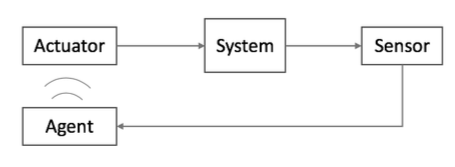
\includegraphics[width=10cm]{event.png}
 	\caption{制御系} \label{image}
\end{figure}\par
これに対するフィードバック制御を考える. 状態変数$s$を観測してアクチュエータに入力信号を送信することを「インタラクション」と呼ぶと,セルフトリガー制御では, 連続的なインタラクションは行わずに, 次のインタラクションを何秒後に行うかをエージェントが決定する. それを数式上で表すため, エージェントの制御則$\pi(s)$は2つの要素からなるベクトル値関数であるとし, 1つ目の要素はアクチュエータに送信する入力$a$,~2つ目の要素は次にインタラクションを行うまでの時間間隔$\tau~(s:秒)$を表すものとする.また, 次のインタラクションを行う時刻までは1つ前のインタラクションで送信した入力$a$を加え続けるものとする(ZOH制御).

\subsection{最適セルフトリガー制御}
最適なセルフトリガー制御則$\pi^{*}$を, 以下のように定義する. 
\begin{align}
	\pi^{*} &= \argmax_{\pi}J(\pi) \label{optimal_policy}\\
	J(\pi) &= \expect_{s_0\in d_0}[V^{\pi}(s_0)] \\
	% V^{\pi}(s_0) &= \sum_{i=0}^{\infty} \gamma^i\{-s_i^{\top}Qs_i-\pi_1(s_i)^{\top}R\pi_1(s_i)+\lambda \pi_2(s_i)\} \\
	V^{\pi}(s_0) &= \sum_{i=0}^{\infty} \gamma^i r^{\pi}_i \label{value} \\
	r^{\pi}_i &= -\int_{T_i}^{T_{i+1}}s(t)^{\top}Qs(t)\textrm{d}t +\tau_ia_i^{\top}Ra_i + \lambda \tau_i, ~T_i = \sum_{l=0}^{i} \tau_l \label{reward}
\end{align}
ここで, $i$はインタラクションの回数を示し, $a_i, \tau_i$はそれぞれ$i$回目のインタラクションでの方策$\pi$の出力であるとする. \par
さて, 一般的に強化学習では, 1ステップ1ステップの行動の良し悪しを評価して方策を更新していく. 
インタラクションとインタラクションの間の区間を「インターバル」と呼ぶと, 式(\ref{value})より, この問題は各インターバルを1ステップとした強化学習問題であると考えることができる. \par

\section{数値実験による課題点の抽出}
上記の問題は, 一般的な強化学習のフレームワークにそのまま落とし込むことができるため, 数値実験を行うことが可能である. 数値実験の結果を通して, 最適セルフトリガー制御の強化学習にどのような課題点があるのかを考察していく.\par
実験環境はOpen-AI Gymのpendulumで, 初期状態が$\theta\sim N(0, \pi), \dot{\theta}\sim U(-\pi,\pi)$となるような環境で行った. またreplay bufferの分散を上げるため,~10秒間の制御を1エピソードと定義し, エピソードを重ねることで経験データを増やしていく. また, pendulumは以下のようなダイナミクスに従っており入力アフィン系の非線型システムである.
\begin{equation}
	\odif{}{t}\begin{pmatrix}\theta \\ \dot{\theta}\end{pmatrix} = 
		\begin{pmatrix}\dot{\theta} \\ \frac{3g}{2l}\sin{\theta} + \frac{3}{ml^2}a \end{pmatrix} \label{pendulum}
\end{equation}

\subsection{初期方策}
学習の初期方策として
\begin{align}
\begin{cases}
	a(s)=a_{0.05}^{*}(s)\\
	\tau(s)=0.2
\end{cases} \label{pi_init}
\end{align}
とする方策$\pi_{\rm{init}}$を用いる.ただし, $a_{0.05}^{*}(s)$はシステム\eqref{pendulum}を,離散化幅$\delta_t=0.05$として離散化したシステムを原点付近で安定化する制御則として与える.

\subsection{学習によって得られた方策}
方策を表現するニューラルネットワークモデルや, 学習率などを工夫することで, 学習を安定的に進めることができた. 方策$\pi_{\rm{init}}$から1000000ステップの学習を行うことで得られた方策を$\pi_{\rm{RL}}$と書くと,~$\pi_{\rm{RL}}$による, とある初期状態からの制御の様子は以下のようになる.
\begin{figure}[h]
	\centering
 	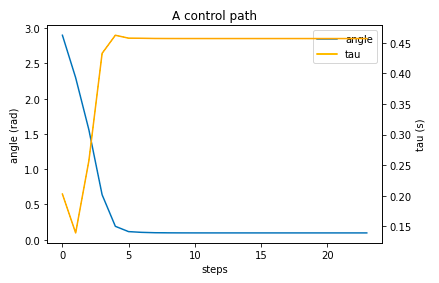
\includegraphics[width=7cm]{self_trigger_log.png}
 	\caption{$\pi_{\rm{RL}}$による制御ログ(角度(rad)と通信間隔(s))} \label{self_trigger_log}
\end{figure}\par
図\ref{self_trigger_log}からは, 原点付近では通信間隔を大きく, そうでない場合は通信間隔を小さく, というふうに適応的に通信間隔を決定している様子が見られる.
\par
この時の評価関数$J(\pi_{\rm{RL}})$の値は
\begin{equation}
	J(\pi_{\rm{RL}}) = 45
\end{equation}
となり, 初期方策$\pi_{\rm{init}}$に対する$J(\pi_{\rm{init}})=-14$を上回った.\par

\subsection{学習の様子}
DDPGでは, 方策$\pi$を表現するactorと, 方策$\pi$の良し悪しを特徴付ける$Q^{\pi}(s,a)$を表すcriticをそれぞれ更新していく. criticは過去の経験データを教師データとして用いる教師あり学習でパラメータを学習する. また, actorはcriticが正しく$Q^{\pi}(s,a)$を近似できていれば(方策勾配の割引分布に関する期待値を除けば)評価関数$J(\pi)$を大きくする方向に正しくパラメータを更新することができる. したがってcriticの学習における損失関数の値を追うことで, DDPGアルゴリズムが方策改善を行えているかどうかおおよそ知ることができる.\par
方策$\pi_{\rm{init}}$から方策$\pi_{\rm{RL}}$を得る1000000ステップの学習では, criticの損失関数がある一定値のまわりの値を取りながら振動しており, 収束していく様子は見られなかった. この原因を考察していく.\par
actorのパラメータ更新には方策勾配\eqref{true_pg}が用いられる. したがって$\nabla_{a}Q(s,a|\omega)$の値は非常に重要である. (データは後で載せますが, )方策$\pi_{\rm{RL}}$でエピソードを数回経験すると, 原点付近の状態を数多く経験していることが確認できる. これは方策勾配の状態$s$に関する期待値が, 原点付近にあることを示しているので, 特に$s=[0,0]$でのcritic~$Q(s,a|\omega)$の, $u=0$の断面を見てみると,
\begin{figure}[h]
	\centering
 	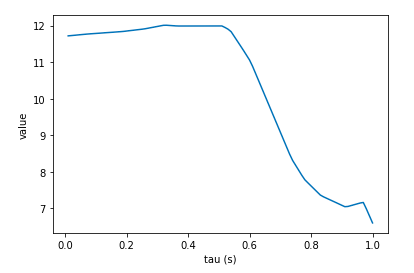
\includegraphics[width=6cm]{tau_gradient_origin.png}
 	\caption{原点で何も入力を加えない時のcriticと$\tau$のグラフ} \label{tau_gradient_origin}
\end{figure}\\
のようになった. このため, $\tau$に関する$Q(s,a|\omega)$の微分値がほぼ0となるため, オプティマイザAdamの性質により, この台の上を振動してしまう. ただし, 微分値がほぼ0となったり, $\tau>0.5$の領域で急激に減少するのは探索不足が原因である(探索雑音を加えすぎると発散してしまう(探索と活用のジレンマ)).\par 
従ってactorが収束しないことになるので, criticも収束しない. そのことを, critic~$Q(s,a|\omega)$のaに$\pi_{\rm{RL}}(s)$を代入した関数(以下$V^{\pi}_{c}(s)$と記載)と, 定義\eqref{value_function}通りの価値関数$V^{\pi}(s)$を図示して比較することで確認していく.
\begin{figure}[h]
	\centering
 	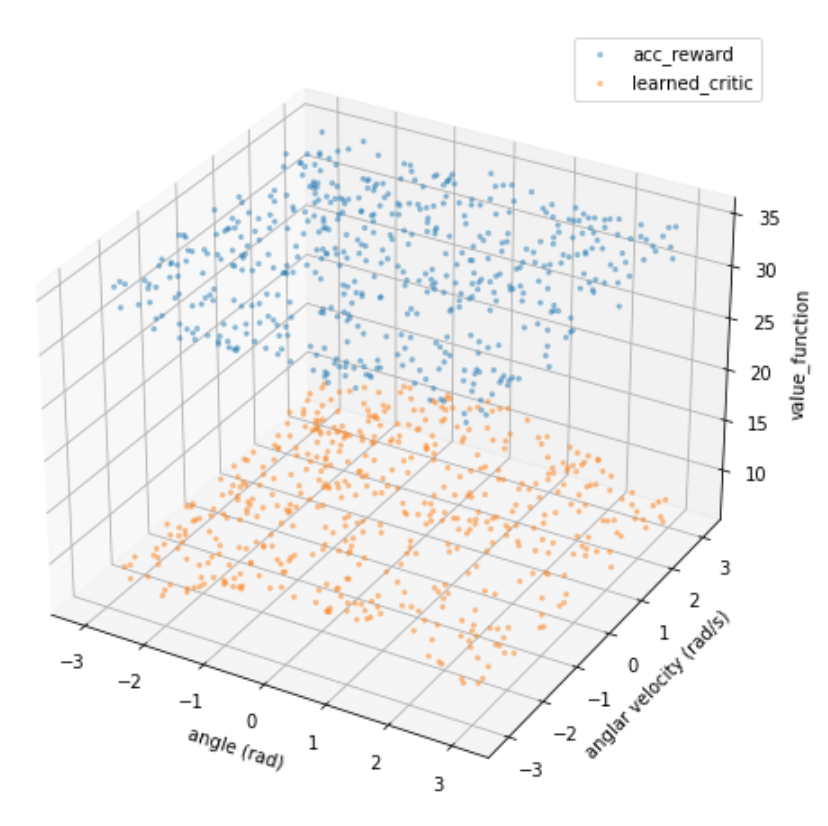
\includegraphics[width=7.5cm]{critic_approximation.png}
 	\caption{DDPGで得られたcriticによる価値関数$V^{\pi}$の近似} \label{critic_approximation}
\end{figure}\\
図\ref{critic_approximation}では橙色に$V^{\pi}_{c}$, 青色に価値関数$V^{\pi}$の関数形を示している(同一色の点を複数プロットすることにより, 関数曲面を表現しているとみてください.) criticが$Q$関数をよく近似できていれば, 橙色の曲面は青色の曲面に一致するため, 近似できているとは結論づけられない.

\section{criticからリアプノフ関数へ}
前節ではactorが収束しないため, criticが$Q$関数を近似する限界があることを示唆した. では, actorを固定して$Q$関数を教師あり学習すれば, criticを収束させられるか確認してみた.

\begin{figure}[h]
	\centering
 	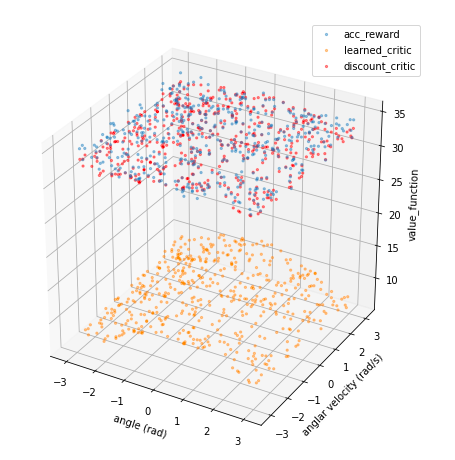
\includegraphics[width=8cm]{supervised_critic.png}
 	\caption{教師あり学習で追加学習したcriticによる価値関数$V^{\pi}$の近似} \label{supervised_critic}
\end{figure}\par
図\ref{supervised_critic}は, 図\ref{critic_approximation}に教師あり学習で学習したcriticに対する$V^{\pi}_{c}$を赤色で追加した図である. 赤色と青色の曲面を比べると, 近いものが得られているので, (価値関数$V$は)近似が可能であると結論づけられる.


\section{$Q$関数とcriticネットワークの比較による, 課題点の抽出}
\subsection{$Q$関数の近似精度}
方策勾配は,
\[\nabla_{\theta}J(\pi_{\theta}) = \expect_{s\sim\rho^{\pi}}[
	\nabla_{\theta}\pi_{\theta}(s)\nabla_{a}Q^{\pi_{\theta}}(s, a)|_{a=\pi_{\theta}(s)}]\]
と書けるので, その計算に用いられるのは$Q^{\pi}(s,a)$の$a$勾配である. 実際の方策勾配の計算には$Q^{\pi}(s,a)$の近似であるcriticネットワーク$Q(s,a|\omega)$を用いるので, $Q^{\pi}(s,a)$と$Q(s,a|\omega)$の$a$に関する勾配が等しいことが望ましい. その性質を満たしているか確認する為, $Q(s,a|\omega)とQ^{\pi}(s,a)$に対して, $s=[0,0]$とした時の関数形を図\ref{critic_q_const_s}に示す.
\begin{figure}[h]
	\centering
 	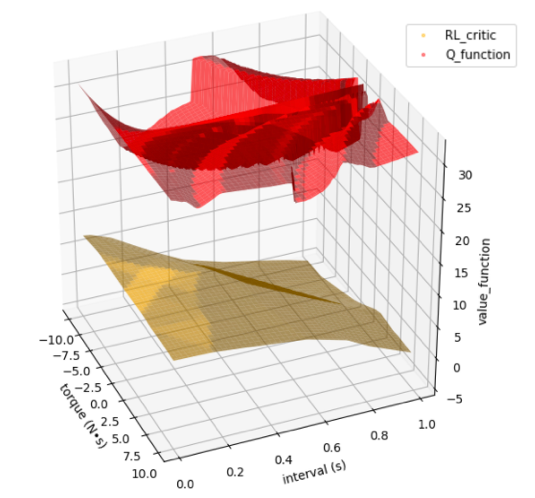
\includegraphics[width=8cm]{critic_q_const_s.png}
 	\caption{$s=[0,0]$に対する$Q$関数の近似精度} \label{critic_q_const_s}
\end{figure}\\
ただし,~$Q^{\pi}$は漸化式
\[Q^{\pi}(s,a) = r(s,a)+\gamma V^{\pi}(s^{\prime})\]
における$V^{\pi}$に, 図\ref{supervised_critic}で得た価値関数を用いることで計算した. 図\ref{critic_q_const_s}から, ~criticは$Q$関数の$a$勾配を近似できていないことが見て取れる.この原因として考えられるのは,
\begin{enumerate}
	\item criticの教師あり学習に用いたデータ組$\{s,a\}$の偏り
	\item ニューラルネットワークの表現力不足
\end{enumerate}
が挙げられる. 特に1つ目について,考察していく.

\subsection{criticの近似と経験データの分散}
criticの近似精度の低さの原因の一つに, criticの教師あり学習に用いたデータ組$(s,a)$の偏りを挙げた. 教師あり学習における教師データの分布がある領域に偏ってしまうと, 当然その分布外の$(s,a)$における関数近似は行うことができない. 経験データの分散を上げる為に多様な入力を試してみることを探索というが, 連続行動空間の強化学習では
\begin{equation}
	a = \pi_{\theta}(s) + e
\end{equation}
のように入力にノイズ$e$を付加してデータ収集を行うのが一般的である. しかしながら, 実際に実験で加えていたノイズは, 非常に小さいものであった. このことが経験データの分布に偏りをもたらしてしまっていると考えられる.\par
さて, criticは損失関数
\[L=\frac{1}{N}\sum_{(s,a)\in E}\{Q(s,a|\omega) - \{r(s,a)+\gamma Q(s,\pi(s)|\omega)\}^2\]
を小さくするように, パラメータ更新をするのであった. ここで, ~$E$は過去の経験データを表す為, その分布に偏りがあったことが, 低い近似精度の原因の一つであると考えられる. 


\subsection{割引分布と探索ノイズ}
では, 探索ノイズを大きくすればそれで良いのか. 答えはNOである. 大きな探索ノイズを加えれば, 経験データ$E$の分布は割引分布$\rho^{\pi}(s)$から大きく乖離することになる. これはどのような問題を引き起こすのか.\par
actorの更新に用いる方策勾配の計算には,~$Q^{\pi}$のcriticによる近似の他にも, 以下のように状態$s$に対する期待値のサンプル平均による近似も用いられる.
\[
\expect_{s\sim\rho^{\pi_{\theta}}}[\nabla_{\theta}\pi_{\theta}(s)\nabla_{a}Q(s, a|\omega)|_{a=\pi_{\theta}(s)}] \simeq \frac{1}{N}\sum_{s\in E}[\nabla_{\theta}\pi_{\theta}(s)\nabla_{a}Q(s, a|\omega)|_{a=\pi_{\theta}(s)}]
\]
よって, 経験データ$E$の分布は割引分布$\rho^{\pi_{\theta}}(s)$に等しいことが望ましい. 従って, 入力に大きなノイズを加えることは,方策勾配の近似に対しては望ましくない操作であると言える.

\subsection{探索と利用のジレンマ}
前節と前々節で確認した探索ノイズに対する2つの要求は互いに相反するのものであり, 強化学習における有名な課題である. 最適セルフトリガー制御の強化学習に対する最後の課題として, このジレンマの最小化に取り組みたい. より具体的には, 効率的な探索ノイズについて考察する.\par
効率的な探索とは, 以下の二つの要求を満たすような探索である.
\begin{enumerate} 
	\item 経験する状態$s$の分布は, 割引分布$\rho^{\pi}(s)$に近いものにしたい
	\item 各状態$s$に対して, 様々な入力$a$を経験したい
\end{enumerate}
前述の通り, 連続行動空間に対する探索には, データ収集時の入力にノイズを加えるという手法が用いられる. このノイズの大きさを適応的に制御することによって, 上記のジレンマを解決する手法を考えたい. 以下ではそれに対する考察を行う.

\subsection{適応的探索ノイズ}
前節で述べたジレンマは, 「入力$a$を変えても,次ステップの状態$s^{\prime}$が大きく変わらない場合」は大きなノイズを加え, 「入力$a$を変えると,次ステップの状態$s^{\prime}$が大きく変わってしまう場合」はノイズは小さくすることによって, 最小化できるのではないかと考えている. \par
例えば, 探索ノイズを正規乱数$\mathcal{N}(0,1)$のスカラー倍として与える場合に, そのスカラー$k$(以下ノイズスケールと記載)を適応的に変化させることを考える. 次ステップの状態$s^{\prime}$は, 現在の状態$s$と入力信号$u$および通信間隔$\tau$の関数として与えられるので, 
\[\pdif{s^{\prime}}{u}, \pdif{s^{\prime}}{\tau}\]
の大きさによって, ~$u,\tau$それぞれに加えるノイズスケール$k_u, k_{\tau}$を適応的に与えれば良い. \par
しかしながら,~$s^{\prime}$の計算にはシステム\eqref{pendulum}が既知である必要があるので, 議論の一般性を失う. そこで, システムに対する必要な知識を緩和することを考える. \cite{ECBF}では, 入力アフィン系
\begin{equation}
	\dot{s} = f(s)+g(s)u
\end{equation}
における$f,g$のリプシッツ連続という性質のみを用いて,  
\begin{equation}
	\|s^{\prime}-s\|\leq \frac{1}{L}\|f(s)+g(s)u\|(e^{L\tau}-1)=\bar{r}(s,u,\tau)
\end{equation}
のように, セルフトリガー制御における状態変化に上界を与えた. これはつまり, 次ステップの状態$s^{\prime}$が
\begin{equation}
	s^{\prime} \in B, B=\{s^{\prime} :\|s^{\prime}-s\|\leq \bar{r}\}
\end{equation}
を満たすことを保証したことになる(図\ref{s_prime}参照).
\begin{figure}[h]
	\centering
 	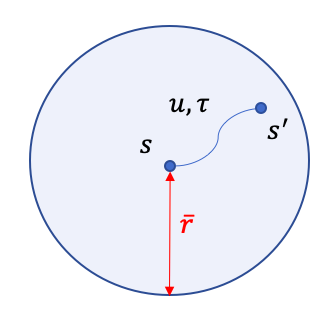
\includegraphics[width=5cm]{s_prime}
 	\caption{セルフトリガー制御における状態変化の上界} \label{s_prime}
\end{figure}\\
この半径$\bar{r}$に対して, 
\[\pdif{\bar{r}}{u}, \pdif{\bar{r}}{\tau}\]
を用いることにより, ノイズの適応的な制御ができないかを考えていきたい.


\begin{thebibliography}{10}
\bibitem{ECBF}
G. Yang, C. Belta, and R. Tron. “Self-triggered Control for Safety Critical Systems Using Control Barrier Functions."  \textit{In American Control Conference (ACC) Philadelphia, USA}, 2019.
 
 \end{thebibliography}
\end{document}